\documentclass[12pt]{beamer}
\usetheme{CambridgeUS}
\usepackage[utf8]{inputenc}
\usepackage[spanish]{babel}
\usepackage{amsmath}
\usepackage{amsfonts}
\usepackage{amssymb}
\usepackage{graphicx}

\author{Kevin Steven García \\ Cesar Andres Saavedra}
\title{Generación de números aleatorios \\ Modelos probabilisticos \\ Pruebas de bondad de ajuste}
%\setbeamercovered{transparent} 
%\setbeamertemplate{navigation symbols}{} 
%\logo{} 
\institute{Universdiad del Valle \\ Estadística \\ Simulación Estadística} 
\subject{} 
\date{Abril 2018}


\begin{document}

\begin{frame}
\titlepage
\end{frame}


\begin{frame}
\frametitle{Introducción}

\begin{block}{\textbf{Distribucion Poisson:} 
~\\La distribución de Poisson es, una de las mas importantes distribuciones de probabilidad discretas, es decir, aquellas de las cuales pueden tomar los valores 0,1,2,3,...,k.  
~\\Cada una de las Variables aleatorias representa el numero total de ocurrencias de un fenómeno durante un periodo de tiempo fijo o en una región fija del espacio y expresa la probabilidad de un numero k de ocurrencias.}
\end{block}
\end{frame}

\begin{frame}
\begin{block}{\textbf{Distribucion Logistica:}
~\\La distribución Logística es una distribución de probabilidad continua cuya función de distribución es la función logística, que aparece en el contexto de la regresión logística. Siendo la regresión logística un instrumento estadístico de análisis multivariado, de uso explicativo y predictivo. Que resulta útil cuando se tiene una variable dependiente dicotomica, atributo de ausencia o presencia que se puntuá con valores de 1 y 0, respectivamente.}
\end{block} 
\end{frame}

\begin{frame}
\frametitle{ Artículos}
\begin{itemize}
\begin{block}{\item\textbf{Evidence in support of seismic hazard following Poisson distribution.\\Pruebas de apoyo al riesgo sísmico tras la distribución Poisson.}}
\end{block} 
\end{itemize}

\begin{itemize}
\begin{block}{\item\textbf{APLICAÇÃO DE REGRESSÃO LOGÍSTICA E ALGORITMOS GENÉTICOS NA ANÁLISE DE RISCO DE CRÉDITO.\\Aplicación de la regresión logística y de los algoritmos genéticos en el análisis del riesgo de crédito.}}
\end{block} 
\end{itemize}
\end{frame}

\begin{frame}
\frametitle{Simulación Distribuciones }
\begin{figure}
\centering
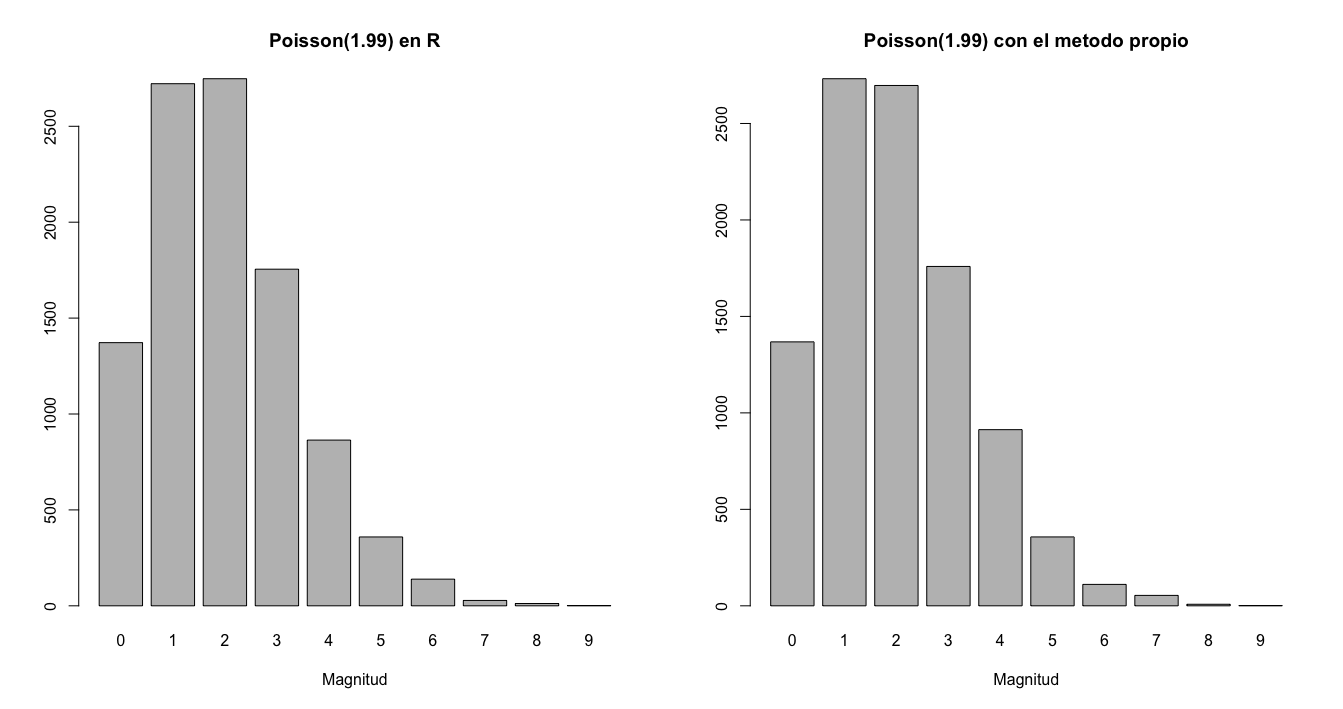
\includegraphics[scale=0.3]{imagenes/Rplot1.png}
\caption{Comparación simulaciones en R y con el método propio de la distribución Poisson($\lambda=1.99$)}\label{figura2}
\end{figure}
\end{frame}

\begin{frame}
\frametitle{Simulación Distribuciones}
\begin{figure}
\centering
\includegraphics[scale=0.3]{imagenes/logic.png}
\caption{Comparación simulaciones en R y con el método de la transformada inversa para la distribución Logistica($a=0,b=2$)}\label{figura2}
\end{figure}
\end{frame}

\begin{frame}
\frametitle{Simulación Pruebas de bondad de ajuste}
\begin{figure}
\centering
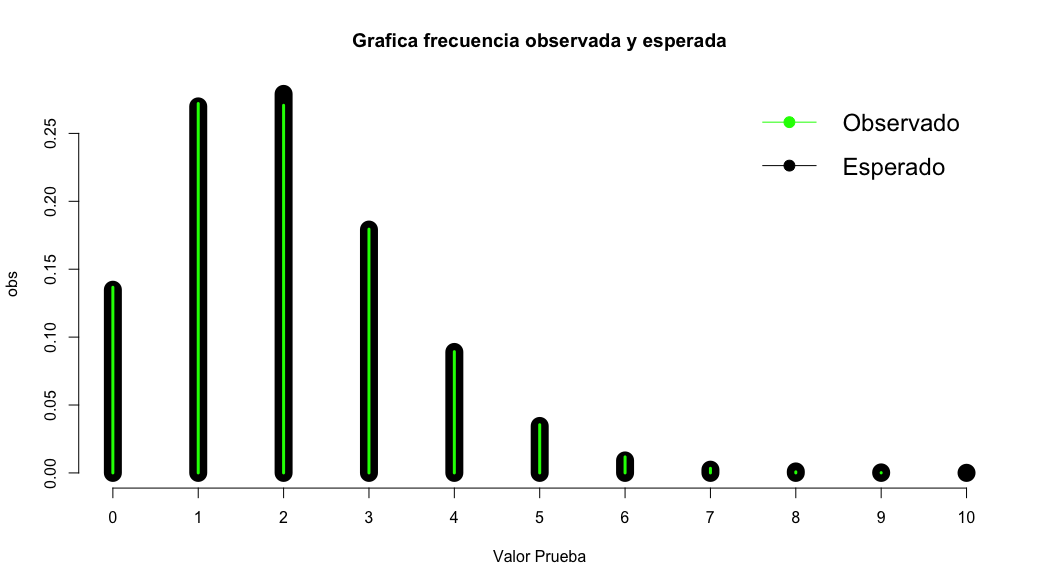
\includegraphics[scale=0.3]{imagenes/poisson.png}
\caption{Frecuencia esperada y observada Poisson $(\lambda=1.99)$)}\label{figura2}
\end{figure}
\end{frame}


\begin{frame}
\frametitle{Simulación Pruebas de bondad de ajuste}
\end{frame}

\begin{frame}
\frametitle{Resultados}
\end{frame}

\begin{frame}
\frametitle{Conclusiones}
\begin{itemize}
\item{}
\item{}
\item{}
\item{}
\item{}
\end{itemize}
\end{frame}

\begin{frame}
\frametitle{Bibliografía}
\begin{block}{\textbf {Statistical distributions, Catherine Forbes, Merran Evans, Nicholas Hastings, Brian Peacock, Fourth edition.}}
\end{block}	
\begin{block}{\textbf {http://www.redalyc.org/html/750/75040605/}}
\end{block}
\begin{block}{\textbf {https://www.sciencedirect.com.bd.univalle.edu.co}}
\end{block}
\end{frame}

\end{document}